%\vspace{1.5pc}
\vspace{1.5pc}
%\section[State of the Art]{State of the Art}
\begin{spacing}{1.5}
	
	Bab ini menjelaskan lebih detail mengenai pustaka relevan dan tinjauan teori dalam penelitian ini. Hal ini bertujuan untuk mereview, mengupdate, mengkritik dan mensintesis literatur, melakukan meta-analisis literatur, melakukan konsepsi ulang dari topik yang direview, dan menjawab pertanyaan spesifik penelitian dari topik yang telah direview dalam literatur \shortcite{Torraco2016}. Struktur pembahasan studi relevan dan tinjauan teori selanjutnya dibagi dalam beberapa hal: pertama, akan dibahas mengenai persamaan gerak fluida dan Navier-Stokes dalam pemodelan laut, termasuk didalamnya grid C Arakawa, dan diskritisasi numerik atas persamaan Navier-Stokes serta kriteria kestabilan dari model. Terakhir, akan dibahas mengenai model iklim yang digunakan.
	
	
\end{spacing}
\vspace{-0.1pc}
\section[Persamaan Gerak Fluida]{Persamaan Gerak Fluida}
\begin{spacing}{1.5}
	
	Persamaan matematika yang mengatur aliran viskoelastik fluida berasal dari persamaan-persamaan hukum konservasi fisika yaitu konservasi massa, momentum dan persamaan konstitutif reologi \shortcite{Alves2021}. Penjabaran dari hukum-hukum tersebut menentukan bagaimana suatu persamaan model hidrodinamika dibuat. Salah satu persamaan fluida yang paling terkenal adalah persamaan Navier-Stokes yang terdiri dari persamaan momentum, persamaan kontinuitas, dan persamaan konservasi densitas \shortcite{Haditiar2020}. Persamaan Navier-Stokes digunakan untuk menggambarkan fluida yang mengalir dan dianggap memiliki pergerakan yang kontinu. Diketahui bahwa hasil pengamatan dari sebuah partikel fluida yang mengalir memiliki sifat-sifat fluida secara umum yaitu kecepatan, temperatur, tekanan dan densitas \shortcite{Rafiq2019,Das2018,Khan2019}. Sebuah partikel fluida diilustrasikan pada Gambar \ref{fig:cube}a, dan \ref{fig:cube}b. Komponen fluida seperti tekanan $p$, kecepatan $u$, dan densitas $\rho$ terletak pada pusat partikel yang bergantung terhadap waktu $(t)$ dan ruang $(x,y,z)$. Sehingga, komponen-komponen tersebut dapat ditulis dalam fungsi $p(x,y,z,t), u(x,y,z,t)$  dan $\rho(x,y,z,t)$. 
	
	Asumsikan bahwa partikel fluida yang diobservasi sangat kecil sehingga sifat fluida pada permukaan kubus dapat diekspresikan secara akurat dengan menggunakan dua suku pertama dari ekspansi deret Taylor, 
	\begin{equation*}
		\sum_{n=0}^{\infty}\frac{f^{n}(a)}{n!}(x-a)^n = f(a)+\frac{f'(a)}{1!}(x-a)+\dots
	\end{equation*} 
	Sebagai contoh, tekanan pada muka $W$ dan $E$, keduanya memiliki jarak $\frac{1}{2}\delta x$ dari posisi partikel di tengah sehingga diperoleh bentuk ekspresi,
	\begin{equation*}
		p-\frac{\partial p}{\partial x}\frac{1}{2}\delta x \quad \text{dan} \quad
		p+\frac{\partial p}{\partial x}\frac{1}{2}\delta x.
	\end{equation*}
	Hal yang sama dapat dilakukan untuk variabel yang lainnya.
	\begin{figure}[H]
		\centering
		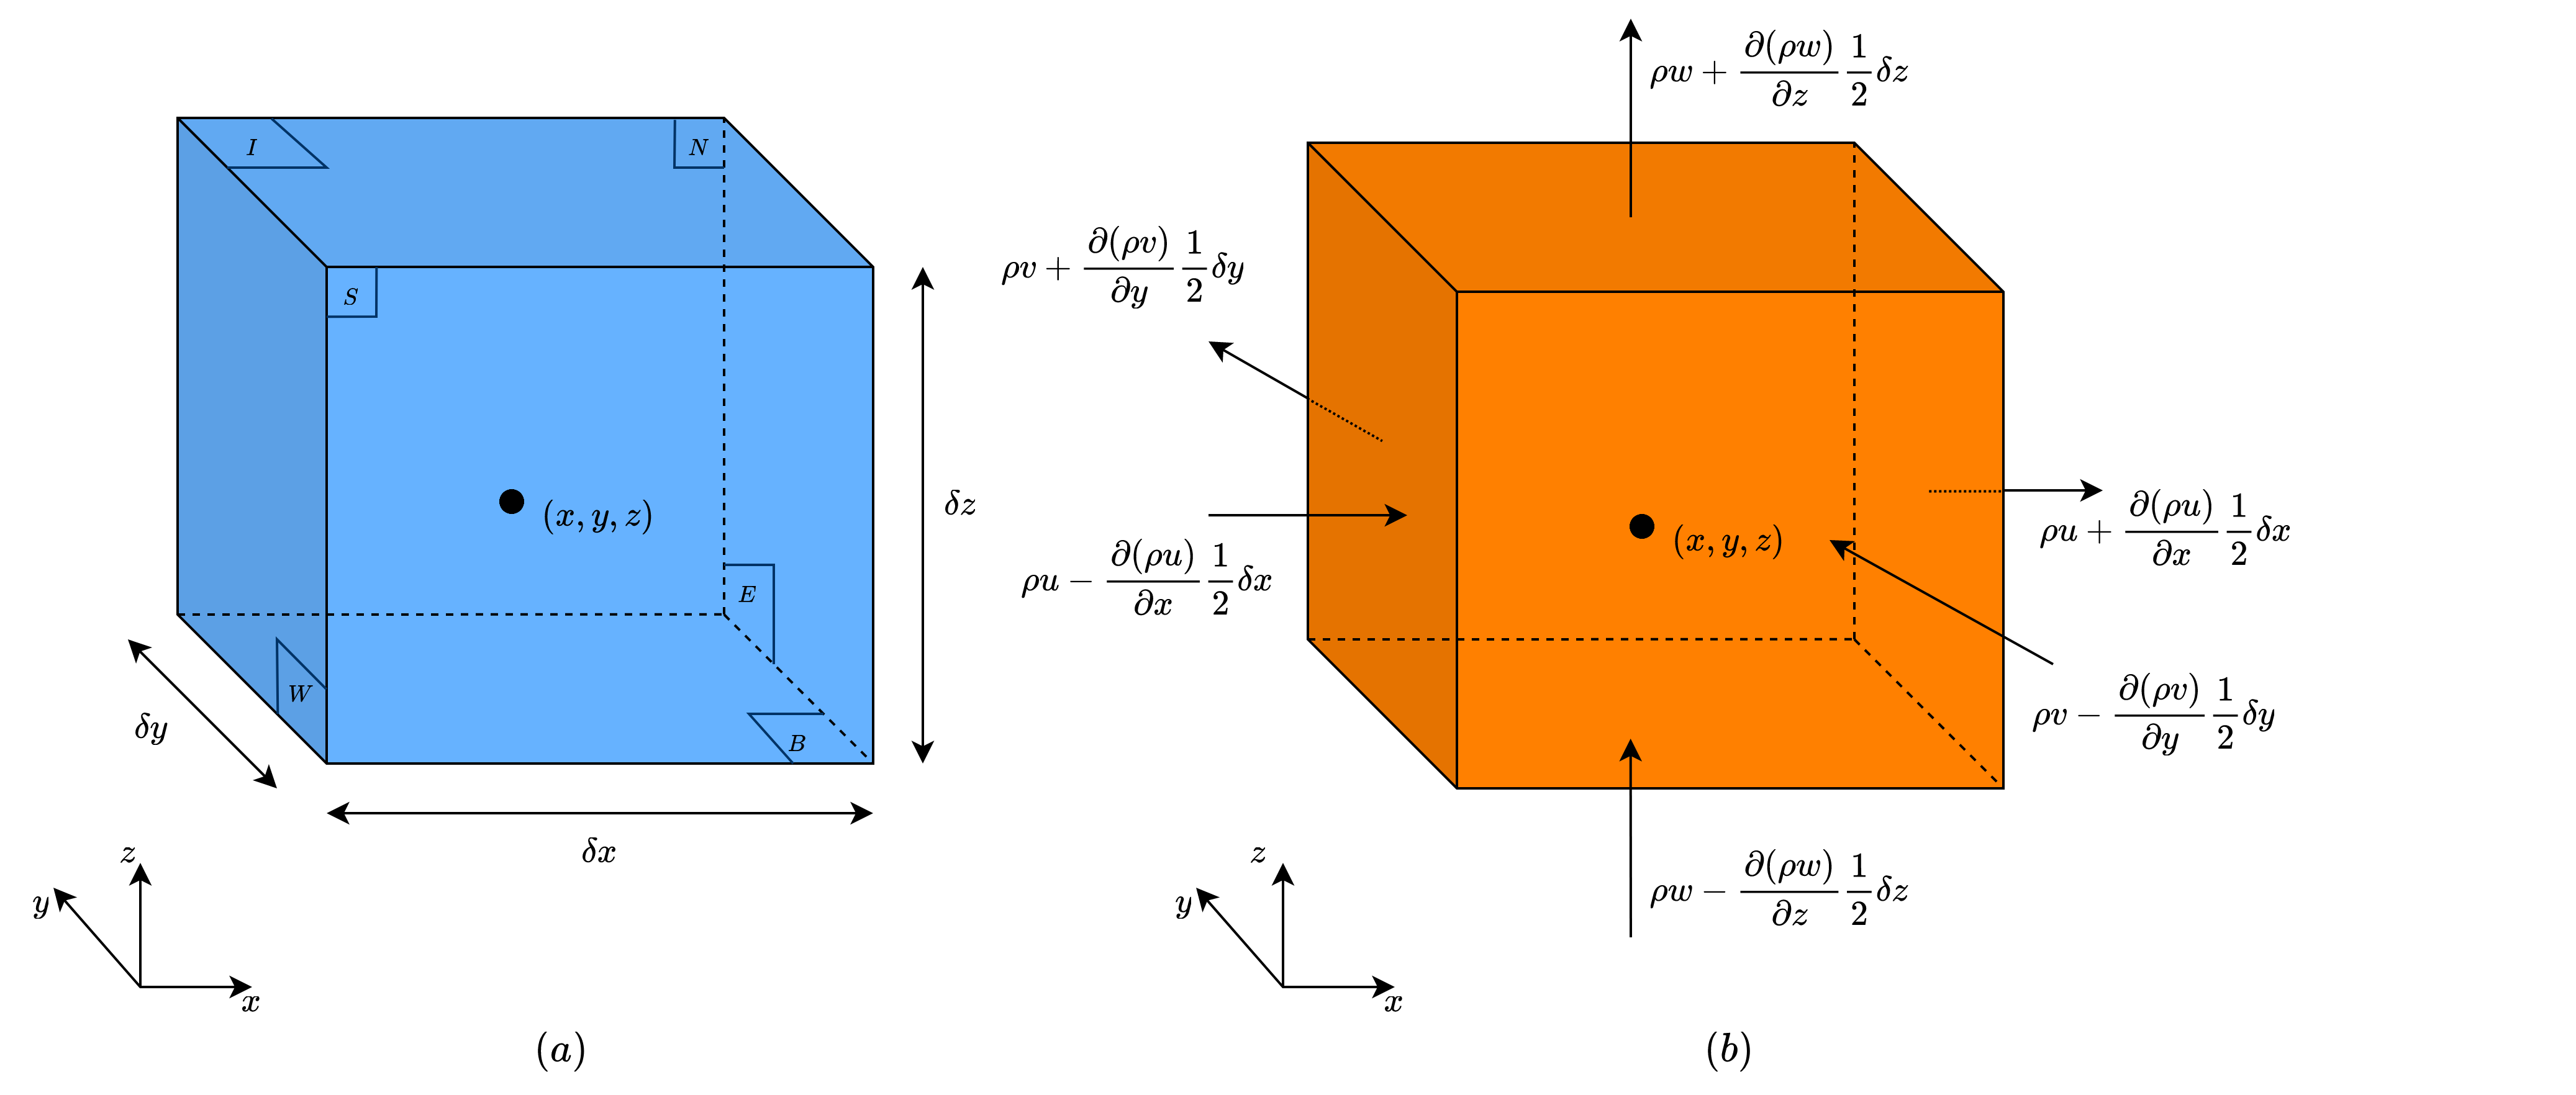
\includegraphics[width=16cm]{contents/cube}
		\caption{(a) Ilustrasi partikel sebagai sifat fisis fluida. (b) Aliran massa jenis masuk dan keluar \protect\shortcite{versteeg2007introduction}}
		\label{fig:cube}
		\medspace
		\small
		Massa jenis dari partikel $\rho(x,y,z,t)$ pada gambar bagian (a) dapat diterjemahkan sebagai aliran yang masuk dan keluar. Pada gambar bagian (b), arah aliran massa jenis pada partikel pusat merupakan jumlahan dari aliran massa jenis masuk dan keluar. Dengan cara yang sama, dapat juga dilakukan untuk tekanan dan kecepatan. 
	\end{figure}
	
\end{spacing}
\vspace{-1pc}
\section[Persamaan Navier-Stokes 3 Dimensi]{Persamaan Navier-Stokes 3 Dimensi}
\begin{spacing}{1.5}
	\par Model sirkulasi laut atau \textit{Ocean General Circulation Models} (OGCM) menggunakan persamaan Navier-Stokes untuk memodelkan fenomena fisis yang terjadi di lautan. Persamaan gerak Navier-Stokes nonhidrostatik dalam model 3-D terdiri dari persamaan momentum, persamaan kontinuitas, dan persamaan konservasi densitas \shortcite{Haditiar2020}. Pada model Navier-Stokes dengan pendekatan nonhidrostatik, tekanan air laut (P) dipecah menjadi dua bagian utama, yaitu: tekanan hidrostatik (p) dan tekanan nonhidrostatik (q)
	\begin{equation}
		P = p+q.
	\end{equation}
	Tekanan p dihitung secara diagnostik dari densitas  dan percepatan gravitasi g seperti pada persamaan berikut 
	\begin{equation}
		\frac{\partial p}{\partial z} = -(\rho - \rho_0)g.
	\end{equation}
	Sedangkan tekanan q dihitung secara prognostik dalam persamaan momentum (implisit). Hal ini karena tekanan q bergantung terhadap sirkulasi arus.
	\par Persamaan momentum lengkap untuk model nonhidrostatik adalah sebagai berikut
	\begin{equation}
		\begin{aligned}
			\frac{\partial u}{\partial t} + \text{adv}(u)-fv &= \frac{-1}{\rho_0}\frac{\partial(p+q)}{\partial x}+\text{diff}(u) \\
			\frac{\partial v}{\partial t} + \text{adv}(v)+fu &= \frac{-1}{\rho_0}\frac{\partial(p+q)}{\partial y}+\text{diff}(v) \\
			\frac{\partial w}{\partial t} +\text{adv}(w) &= \frac{-1}{\rho_0}\frac{\partial(q)}{\partial y}+\text{diff}(w).
		\end{aligned}	
	\end{equation}
	\par Dengan $\text{adv}(\psi)=u\frac{\partial \psi}{\partial x}+v\frac{\partial \psi}{\partial y}+w\frac{\partial \psi}{\partial z}$ adalah persamaan adveksi dan $\text{diff}(\psi)=\frac{\partial}{\partial x}(A_{H} \frac{\partial \psi}{\partial x})+\frac{\partial}{\partial y}(A_{H} \frac{\partial \psi}{\partial y})+\frac{\partial}{\partial z}(A_{Z} \frac{\partial \psi}{\partial z})$ adalah persamaan difusi dengan $A_H$ dan $A_Z$ koefisien gesekan eddy horizontal dan vertikal. Kecepatan arus dalam sistem koordinat Cartesian 3-D didefinisikan dengan u,v, dan w. Waktu didefinisikan dengan t, parameter Coriolis dengan f, dan densitas air laut referensi dengan $\rho_0$.
	
	Konservasi volume diekspresikan oleh persamaan kontinuitas untuk fluida yang tak termampatkan,
	\begin{equation}
		\frac{\partial u}{\partial t} + \frac{\partial v}{\partial t} + \frac{\partial w}{\partial t} = 0.
	\end{equation}
	Berdasarkan persamaan kontinuitas (2.4), tekanan dinamis pada lapisan permukaan dapat dihitung dengan persamaan berikut
	\begin{equation}
		\frac{\partial q_s}{\partial t} = \rho_0 g_i \times \left( \frac{(\partial \left(H \langle u \rangle \right)} {\partial x} + \frac{(\partial \left(H \langle v \rangle \right)} {\partial y}\right)
	\end{equation}
	dengan $q_s = \rho_0 g \eta$. Disini $\rho_0$ adalah densitas air laut referensi, dan $\eta$ adalah elevasi permukaan laut, $H$ adalah total kedalaman laut, dan $<.>$ adalah operator rata-rata vertikal.
	\par Densitas air laut bergantung pada temperatur, salinitas, dan tekanan. Selanjutnya asumsikan bahwa air laut hanya bergantung linear terhadap temperatur dan salinitas, serta difusifitas \textit{eddy} untuk temperatur dan salinitas sama. Persamaan konservasi densitas diberikan oleh,
	\begin{equation}
		\frac{\partial \rho}{\partial t} + \text{adv}(\rho) = \text{diff}(\rho).
	\end{equation}
	
	Dalam aplikasinya, persamaan Navier-Stokes tidak hanya digunakan untuk memodelkan laut, tapi juga merambah ke bidang pemodelan cuaca \shortcite{Rohli2021}, aliran air dalam pipa \shortcite{Ouchiha2012} dan aliran udara di sekitar sayap pesawat \shortcite{Tulus2019}. Dalam bentuk persamaan lengkap dan simplifikasi, persamaan ini juga dapat digunakan untuk mendesain kereta api \shortcite{Croquer2020}, pesawat terbang \shortcite{Chau2021}, dan mobil \shortcite{Ambarita2018}. Terdapat juga studi tentang aliran darah \shortcite{Gill2021}, desain stasiun pembangkit listrik \shortcite{Yang2019}, dan analisis polusi udara \shortcite{Issakhov2022}. 

\subsection[Diskritisasi Numerik]{Diskritisasi Numerik}
\subsubsection[Arakawa C grid]{Arakawa C grid}
	Diskritisasi grid di bidang horizontal dapat dibedakan menjadi grid persegi (\textit{rectiliniear}) Gambar \ref{fig:grid}a dan grid lengkung (\textit{curvlinear}) Gambar \ref{fig:grid}b, di bidang vertikal berupa grid level z (\textit{z-coordinates}) Gambar \ref{fig:grid}c dan grid level s (\textit{$\sigma$-coordinate}) Gambar \ref{fig:grid}d \shortcite{Delandmeter2019}.
	
	\begin{figure}[H]
		\centering
		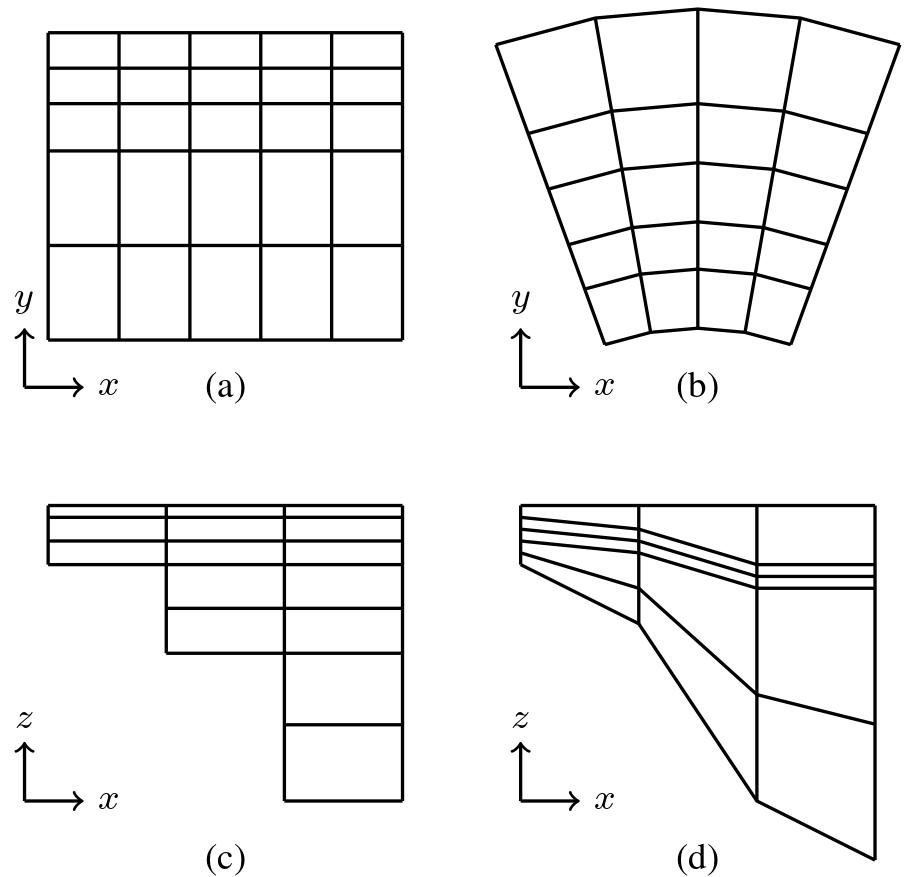
\includegraphics[width=7cm]{contents/grid.jpg}
		\caption{Diskritisasi grid dalam Parcels. Di bidang horizontal: (a) grid persegi, (b) grid lengkung, di bidang vertikal: (c) grid level z, (d) grid level s \protect\shortcite{Delandmeter2019}}.
		\label{fig:grid}
	\end{figure}
	
	Dalam aplikasinya, beberapa software pemodelan laut mengimplementasikan grid bertingkat (\textit{staggered grid}) yang diperkenalkan oleh \shortciteNP{ARAKAWA1977}, yaitu grid A, B dan C. Lebih lanjut, antara grid A, dan grid C terdapat perbedaan fundamental yaitu letak penyimpanan simpul variabel (lihat Gambar \ref{fig:arakawa}), sedangkan grid B dapat dianggap sebagai peralihan dari grid A ke grid C dan perbedaan tipe model grid ini menjadi penting dikarenakan peningkatan kapasitas komputasi yang stabil di banyak pusat pemodelan iklim telah mengantarkan periode transisi untuk model laut global  \shortcite{Barham2018,Delandmeter2019}. 
	
	\begin{figure}[H]
		\centering
		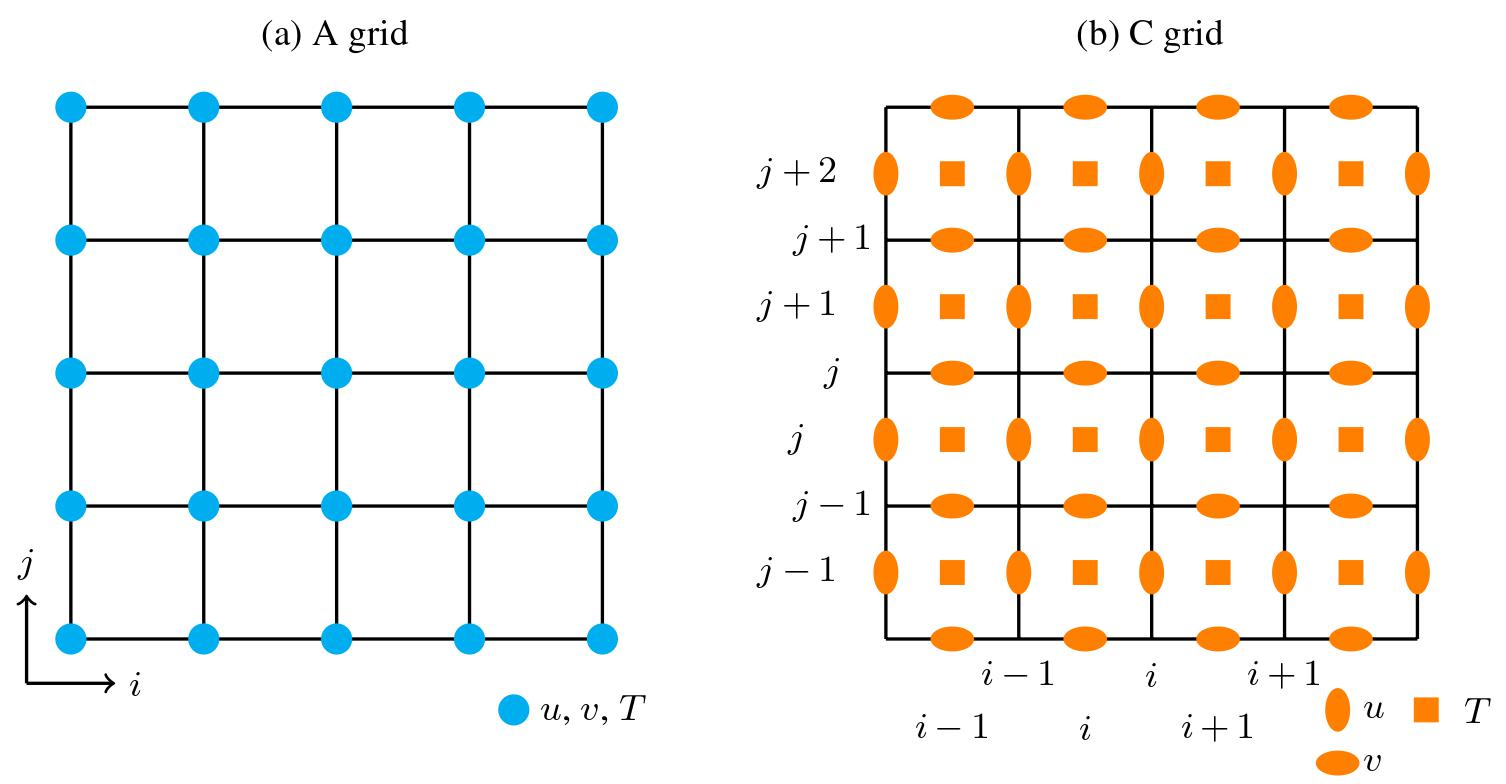
\includegraphics[width=13cm]{contents/arakawa.jpg}
		\caption{Grid Arakawa: (a) Grid A dan (b) Grid C \protect\shortcite{Delandmeter2019}}
		\label{fig:arakawa}
		\medspace
		\small
		Grid A adalah satu-satunya \textit{unstaggered grid} dalam grid Arakawa dimana variabel-variabelnya (\textit{zonal velocity (u), meridional velocity (v), tracers (T)}) hanya terdapat pada titik sudut grid, berbeda dengan grid C yang berada di sisi dan tengah grid. $i$ dan $j$ adalah indeks yang merepresentasikan variabel kolom dan baris dimana variabel disimpan.
	\end{figure}
\subsubsection[Solusi Nonhidrostatik dari Persamaan Momentum]{Solusi Nonhidrostatik dari Persamaan Momentum}
	Dari persamaan 2.4 dan dengan aturan perkalian turunan, suku adveksi untuk parameter sembarang $B$ dapat dituliskan sebagai,
	\begin{equation*}
		u\frac{\partial B}{\partial x} + v\frac{\partial B}{\partial y} + w\frac{\partial B}{\partial z} = \frac{\partial (uB)}{\partial x} + \frac{\partial (vB)}{\partial y} + \frac{\partial (wB)}{\partial z} - B\left(\frac{\partial u}{\partial x} + \frac{\partial v}{\partial y} + \frac{\partial w}{\partial z}\right).
	\end{equation*}
	
	Solusi dari tekanan hidrostatik $q$ dipecah menjadi komponen eksplisit dan implisit sehingga,
	\begin{equation*}
		q \Rightarrow q^n + \Delta q^{n+1}
	\end{equation*}
	Untuk persamaan momentum 3-D, persamaan poisson untuk $\Delta q$ yang bersesuaian adalah
	\begin{equation}\label{eq:poisson}
		\begin{aligned}
			a_e \Delta q_{i,j,k+1}^{n+1} + a_w \Delta q_{i,j,k-1}^{n+1} + a_n \Delta q_{i,j+1,k}^{n+1} + a_s \Delta q_{i,j-1,k}^{n+1} \; + \\
			a_b \Delta q_{i+1,j,k}^{n+1} + 
			a_t \Delta q_{i-1,j,k}^{n+1} -
			a_o \Delta q_{i,j,k}^{n+1} = q_{i,j,k}^{*}
		\end{aligned}
	\end{equation}
	dengan nilai-nilai koefisien,
	\begin{equation}
		\begin{aligned}
			a_e &= a_w = \frac{\Delta z}{\Delta x} \\
			a_n &= a_s = \frac{\Delta z \Delta x}{(\Delta y)^2} \\
			a_e &= a_w = \frac{\Delta x}{\Delta z} \\
			a_o &= a_e + a_w + a_n + a_s + a_b + a_t.
		\end{aligned}
	\end{equation}
	Ruas kanan dari \ref{eq:poisson} merepresentasikan divergensi nilai tebakan pertama dari kecepatan, 
	\begin{equation*}
		\begin{aligned}
		q_{i,j,k}^{*} = \frac{\rho_o}{\Delta t}\left[(u_{i,j,k}^{*}-u_{i,j,k-1}^{*})\Delta z +  (v_{i,j,k}^{*}-v_{i,j,k-1}^{*})\frac{\Delta x \Delta z}{\Delta y}+(w_{i,j,k}^{*}-w_{i,j,k-1}^{*})\Delta x\right].
		\end{aligned}
	\end{equation*}
	Selanjutnya, nilai tebakan pertama dari komponen kecepatan dalam persamaan terakhir dihitung dengan cara,
	\begin{equation}
		\begin{aligned}
			u_{i,j,k}^{*} &= \cos(\alpha)u_{i,j,k}^{n}+\sin(\alpha)v_{u}^{n} - \Delta t \; \text{adv}(u) + \Delta t F_{u}^{n}\\
			v_{i,j,k}^{*} &= \cos(\alpha)v_{i,j,k}^{n}+\sin(\alpha)u_{v}^{n} - \Delta t \; \text{adv}(v) + \Delta t F_{v}^{n}\\
			w_{i,j,k}^{*} &= w_{i,j,k}^{n} - \Delta t \; \text{adv}(w) + \Delta t F_{w}^{n}
		\end{aligned}
	\end{equation}
	dengan $\alpha = \Delta tf, \; u_v \;\text{dan}\;v_u$ adalah nilai $u$ dan $v$ yang diinterpolasi pada titik grid $v$ dan $u$. Nilai $F_{u}^{n}, F_{v}^{n},\;\text{dan}\;F_{w}^{n}$ diberikan oleh,
	\begin{equation}
		\begin{aligned}
			F_{u}^{n} &=-\frac{1}{\rho_o \Delta x}(p_{i,j,k+1}^{n}-p_{i,j,k}^{n}+q_{i,j,k+1}^{n}-q_{i,j,k}^{n})+\text{diff}(u)\\
			F_{v}^{n} &=-\frac{1}{\rho_o \Delta y}(p_{i,j+1,k}^{n}-p_{i,j,k}^{n}+q_{i,j+1,k}^{n}-q_{i,j,k}^{n})+\text{diff}(v)\\
			F_{w}^{n} &=-\frac{1}{\rho_o \Delta x}(q_{i-1,j,k}^{n}-q_{i,j,k}^{n})+\text{diff}(w)
		\end{aligned}
	\end{equation}
	dengan diff($u$), diff($v$), dan diff($w$) menunjukkan momentum difusi. Setelah iterasi \textit{Successive Over-Relaxation} (SOR) telah terkumpul untuk akurasi tekanan yang ditentukan, nilai-nilai komponen kecepatan pada tingkat waktu berikutnya $(n+1)$ diberikan oleh,
	\begin{equation}
		\begin{aligned}
			u_{i,j,k}^{n+1} &= u_{i,j,k}^{*}-\frac{\Delta t}{\rho_o \Delta x}(\Delta q_{i,j,k+1}^{r} - \Delta q_{i,j,k}^{r})\\
			v_{i,j,k}^{n+1} &= v_{i,j,k}^{*}-\frac{\Delta t}{\rho_o \Delta y}(\Delta q_{i,j+1,k}^{r} - \Delta q_{i,j,k}^{r})\\
			w_{i,j,k}^{n+1} &= w_{i,j,k}^{*}-\frac{\Delta t}{\rho_o \Delta z}(\Delta q_{i-1,j,k+1}^{r} - \Delta q_{i,j,k}^{r})\\
		\end{aligned}
	\end{equation}
\subsection[Kriteria Kestabilan]{Kriteria Kestabilan}
	Kriteria stabilitas CFL (Courant-Friedrichs-Lewy) terkait dengan adveksi dari properti yang diberikan, dirumuskan sebagai
	\begin{equation}
		\Delta t \leq min\left(\frac{\Delta x}{u},\frac{\Delta y}{v},\frac{\Delta z}{w}\right).
	\end{equation}
	Terkait dengan perambatan gelombang gravitasi permukaan, kriteria kestabilan diberikan oleh
	\begin{equation}
		\Delta t \leq \frac{min(\Delta x,\Delta y)}{\sqrt{2gh_{max}}}.
	\end{equation} 
	dengan $h_{max}$ adalah kedalaman air maksimum dari domain model.
\end{spacing}
\vspace{-0.1pc}
\section[Model Iklim]{Model Iklim}
\begin{spacing}{1.5}
	Aplikasi deret waktu (\textit{time series}) banyak melibatkan data yang menunjukkan siklus musiman. Contoh yang paling umum digunakan adalah data cuaca. Dalam penelitian \shortciteNP{Haridhi2016}, model nonlinear regresi (Pers. \ref{eq:nrl}) digunakan untuk mengkarakterisasi hubungan antara SST (\textit{sea surface temperature}) dan ND (\textit{net deployment}) - penyebaran jaring nelayan pukat cincin tradisional. Untuk menvalidasi temuan ini, mereka menggunakan persamaan siklus musiman \citeA[p. 793]{crawley2012r} dan mencari korelasi antara data SST dan data meteorologi. Dilain hal, \shortciteNP{Ikhwan2022} dalam penelitiannya mengkaji tentang kedalaman lapisan campuran (MLD) di laut Andaman menggunakan data salinitas (SSS) dari model 3-D CMEMS (\textit{Copernicus Marine Environment Monitoring Service}). Model iklim digunakan untuk mengidentifikasi dan memvalidasi jumlah musim MLD dalam setahun. Persamaan nonregresi linear \shortcite{Haridhi2016} diformulasikan dalam bentuk ,
	\begin{equation}\label{eq:nrl}
		y = b_1 + b_2(\sin(b_3x+b_4))
	\end{equation}
	dengan $b_1$ adalah konstanta pergeseran vertikal, $b_2$ adalah amplitudo gelombang sinus, $b_3$ adalah frekuensi, x adalah variabel waktu, dan $b_4$ adalah fase.
	Persamaan untuk siklus musiman \shortcite[p. 793]{crawley2012r} diberikan oleh,
	\begin{equation}
		y = \alpha + \beta \sin(2\pi t)+\gamma \cos(2\pi t) + \epsilon
	\end{equation}
	dengan adalah $\alpha$ konstanta pergesaran vertikal, $\beta$ adalah amplitude dari gelombang sinus, $\gamma$ adalah amplitude dari gelombang kosinus, $t$ adalah waktu, dan $\epsilon$ adalah elemen residual yang mungkin mewakili komponen white-noise tidak beraturan dalam proses yang mendasari data.
\end{spacing}
\vspace{-0.1pc}
\section[Kedalaman Lapisan Campuran]{Kedalaman Lapisan Campuran}
\begin{spacing}{1.5}
	Laut dan atmosfer berinteraksi dengan permukaan lautan. Gaya permukaan dari atmosfer dan matahari menentukan pola keseluruhan dari suhu permukaan laut (SST). SST yang tinggi pada daerah tropis disebabkan oleh pemanasan (sedikit lebih tinggi dari $29^\circ$C di daerah tropis yang paling hangat) dan SST yang rendah pada daerah latitude atau lintang tinggi disebabkan oleh pendinginan (sekitar $-1.8^\circ$C di daerah pembentuk es, dengan variasi musiman terutama
	terlihat jelas di lintang menengah hingga tinggi). Struktur dari potensial temperatur vertikal dapat dibagi menjadi 3 zona mayor: (1) lapisan campuran (\textit{mixed layer}), (2) lapisan termoklin, dan (3) lapisan abisal. Struktur dari lapisan ini khas untuk daerah lintang rendah dan menengah dengan SST tinggi. Lebih lanjut, 2 zona pertama berada di lapisan paling atas lautan, sedangkan zona temperature yang ketiga berada di lapisan menengah, dalam, dan bawah lautan. Di lintang tinggi di mana SST rendah, struktur ini berbeda, dan dapat memiliki lapisan campuran, suhu minimum vertikal dan maksimum di bawah permukaan laut.
	
	\begin{figure}[H]
		\centering
		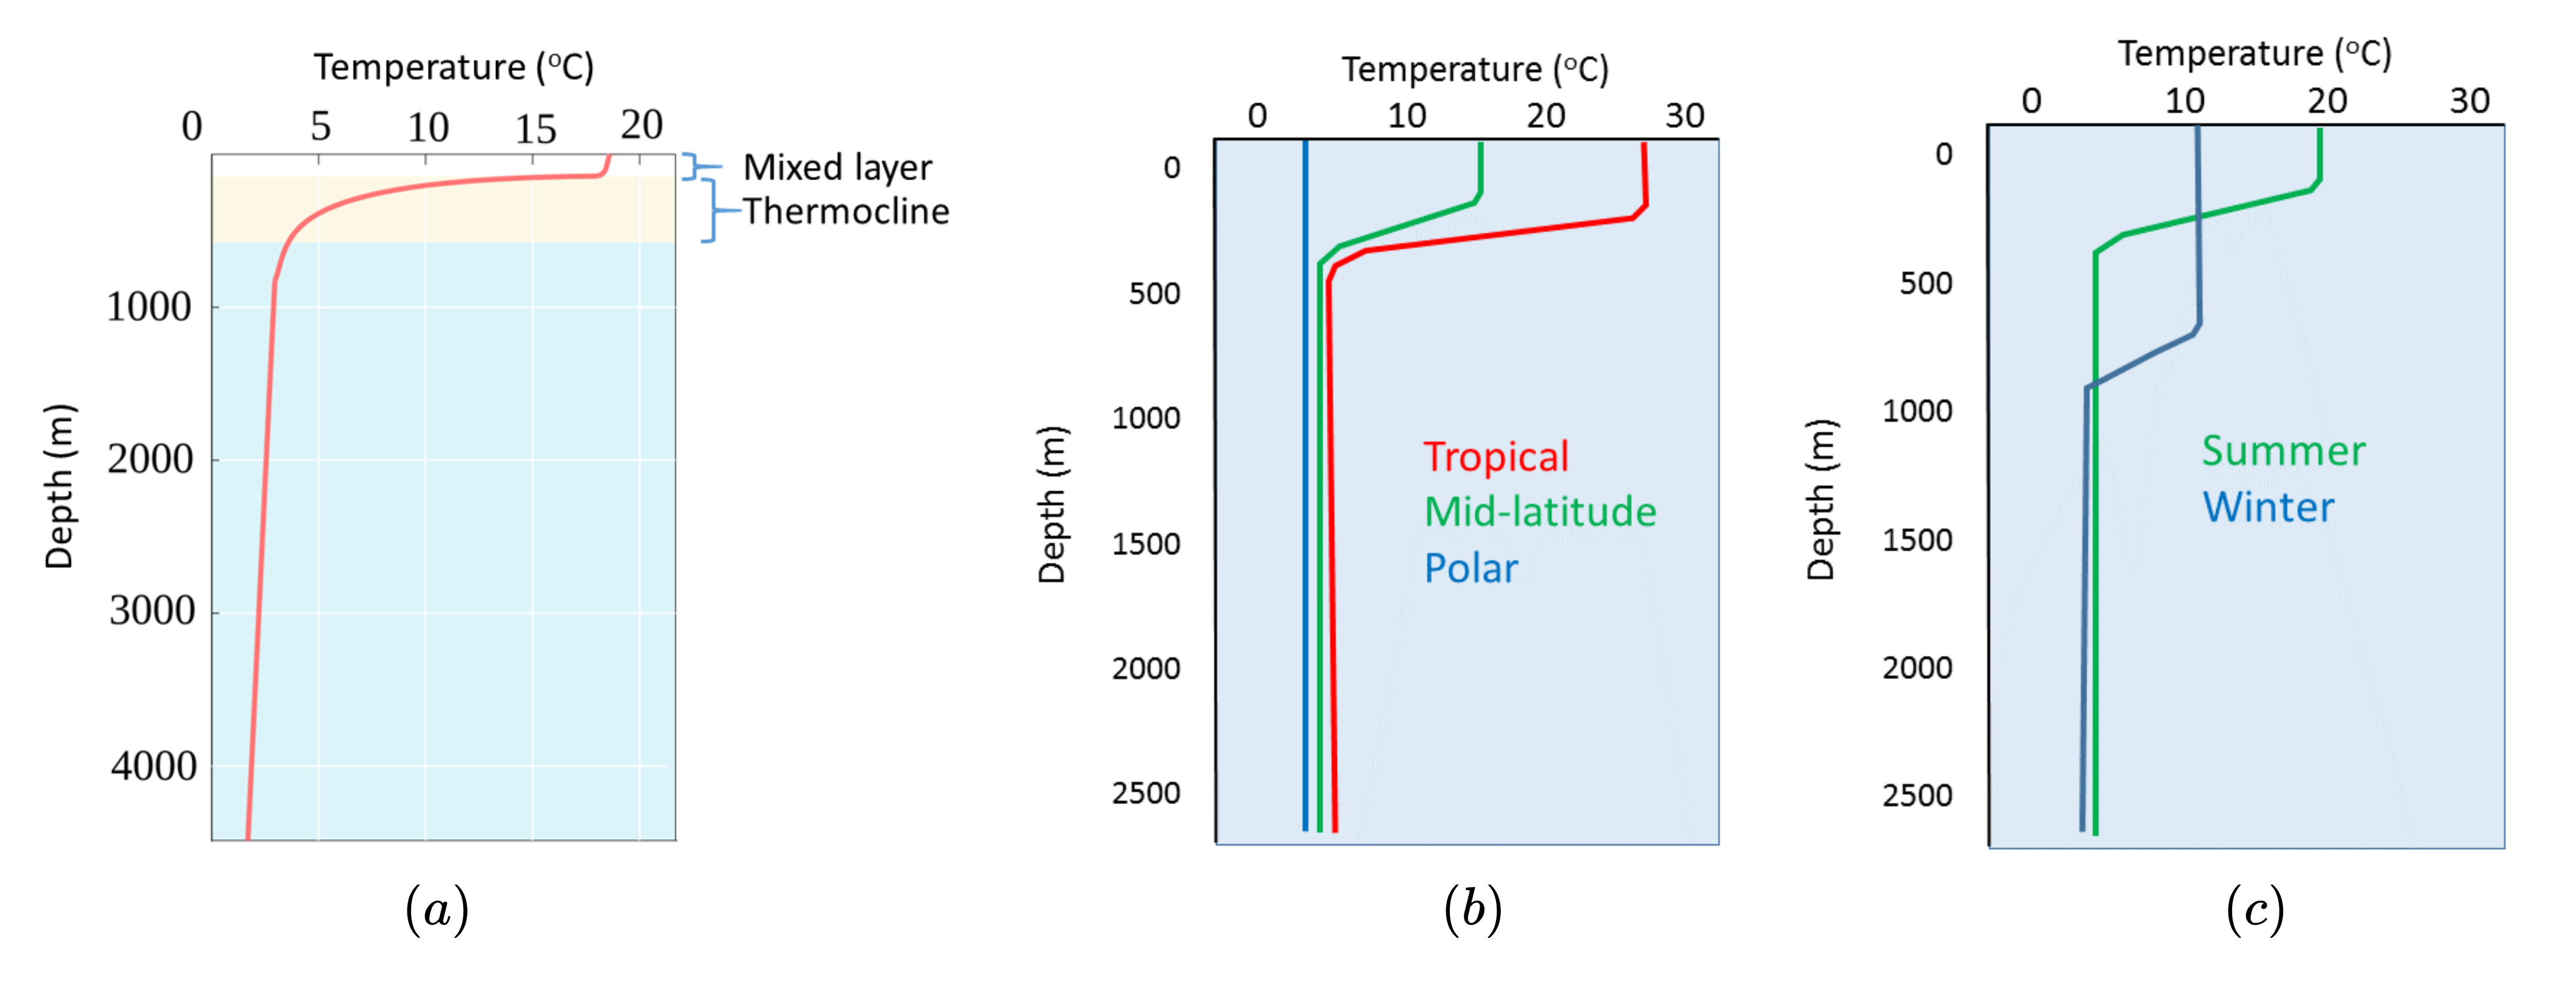
\includegraphics[width=13cm]{contents/mld_theory}
		\caption{Profil suhu potensial ($^\circ$C)/kedalaman (m) tipikal untuk laut terbuka di (a) Pasifik Utara bagian barat tropis ($5^\circ$LU), (b) Pasifik Utara subtropis barat dan timur ($24^\circ$LU), dan ( c) Pasifik Utara subkutub barat ($47^\circ$LU) \protect\shortcite[p. 71]{talley2011descriptive}}
		\label{fig:mld_theory}
	\end{figure}
	Lapisan campuran (\textit{mixed layer} (ML)) adalah lapisan permukaan dengan sifat yang relatif tercampur dengan baik, khususnya di penghujung malam (siklus diurnal) dan di musim dingin (siklus musiman). Pada musim panas di lintang rendah, ML bisa jadi sangat tipis atau bahkan tidak ada sama sekali. Pada musim dingin di lintang menengah hingga tinggi, dan di daerah konveksi dalam yang terisolasi, ML dapat memiliki ketebalan hingga 2000 m. Sebagai tambahan informasi, Lapisan ini bercampur dengan angin dan kehilangan daya apung karena pendinginan atau penguapan (evaporasi) di permukaan laut. ML tidak tercampur oleh pemanasan dan presipitasi di permukaan laut dan oleh sirkulasi di dalam lapisan campuran yang memindahkan air campuran yang berdekatan dengan sifat yang berbeda satu sama lain.
	
	Lapisan termoklin adalah zona vertikal dengan penurunan temperatur yang cepat dengan kedalaman kira-kira 1000 m. Dalam lapisan abisal, antara termoklin dan bawah laut, nilai potensial temperatur menurun secara perlahan. Di lintang tinggi, suhu minimum dekat permukaan (lapisan dikothermal) sering ditemukan, sisa dari lapisan campuran musim dingin yang "tertutup" dengan air yang lebih hangat di musim lain (Gambar \ref{fig:mld_theory}c); suhu maksimum yang mendasari (lapisan mesothermal) dihasilkan dari adveksi air dari lokasi yang agak lebih hangat. Struktur suhu ini stabil karena ada stratifikasi salinitas yang kuat, dengan air tawar di lapisan permukaan. Suhu tipikal di garis lintang subtropis adalah $20^\circ$C di permukaan, $8^\circ$C pada 500 m, $5^\circ$C pada 1000 m, dan $1-2^\circ$C pada 4000 m. Semua nilai ini dan bentuk sebenarnya dari profil suhu adalah fungsi dari garis lintang, seperti yang ditunjukkan oleh tiga profil yang berbeda pada Gambar \ref{fig:mld_theory}.
	
	Lebih lanjut, di semua wilayah pemanasan musim semi dan musim panas menghasilkan lapisan hangat tipis yang menutupi lapisan campuran musim dingin. Di daerah subtropis barat serta daerah lain, sering ada dua termoklin dengan lapisan yang kurang berlapis (lebih isotermal) (termostat) di antara keduanya, semuanya di atas 1000 m (Gambar \ref{fig:mld_theory}b). Di beberapa daerah lapisan campuran lain ditemukan di bagian paling bawah ("lapisan batas bawah") dan dapat mencapai ketebalan 100 m.
\end{spacing}
\vspace{-0.1pc}
%\section[Parameter Meteorologi]{Parameter Meteorologi}
%\begin{spacing}{1.5}
%
%\end{spacing}
